\chapter{Data structures}\label{chapter:datastructures}

\section{Describing data}

Data can be described as a collection of elements, representing a logical piece of information. A data element itself is of a specific data type which is an ordered set containing one or more attributes or fields. The size of this set is referred to as the dimensionality of the data. Different types of data will differ in the combination of their dimensionality and the type of these attributes. We distinguish between three different general kinds of attributes \cite{Shirley:2009:FCG:1628957}:
\begin{itemize}
	\item \textbf{Quantitative} : numerical data attributes on which arithmetic can be applied.
	\item \textbf{Ordered} : an enumeration that has a definite order.
	\item \textbf{Categorical} : data attributes that has no specific ordering, and is distinguished by name only.
\end{itemize}

% Collections = interfaces determining data access
% -> underlying implementation:
%		+ data representation :
% 		1. array
%			2. recursive
%		+ data access (and meta data for speed up)
%			- using algorithms
%			- algorithm determines efficiency in each scenario (read, write,...) (add scenario's to the text ~ use cases)

The collection of elements that represents our data, has a certain structure. This data structure may vary and each variation has very specific advantages and disadvantages. This makes the choice for one data structure or another a significant design choice that have a great impact on the performance of an algorithm and by the extension the computer program of which it is a part.

Data structures are data types themselves, offering a specific public programming interface with an internal implementation. Two aspects drive the implementation of a data structure:
\begin{enumerate}
	\item \textbf{Internal data representation} : The data within the data structure is stored in some way, for example an array or recursive structure.
	\item \textbf{Internal data access algorithms} : To implement the methods of the interface, possibly certain meta-data is required, e.g., start and end indices, and algorithms to access the internal data in a consistent and efficient way.
\end{enumerate}

In the next paragraphs we discuss arrays and recursive data structures.


\subsection{Arrays}

An array is an indexed sequence of elements. The first data element has the index zero, and the index of the last element is equal to the length of the sequence minus one. In many programming languages it is a primitive data type and forms the basis of many data structure implementations. An array has a fixed size and its slots can be directly accessed through their associated index. The data elements in an array are all of the same type. Figure \ref{fig:array} shows an example of an array of integers.

\begin{figure}
	\begin{center}		
		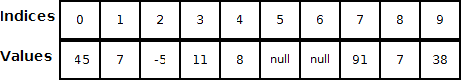
\includegraphics[width=0.6\columnwidth]{img/programming-fundamentals/array}
		\caption{An array of integers with length = $10$. The array has as its first element, i.e., at index $0$, the integer $45$, as last element, i.e., at index $9$, the number $38$. The array also contains two $null$ values, which are default values that don't represent a specific data element.}
		\label{fig:array}
	\end{center}
\end{figure}

A two dimensional array can be constructed as an array of arrays. If all arrays within the including array are of the same length, the resulting data structure is a matrix. This way $N$-dimensional structures can be created.

Arrays can also be thought of as vectors or points within a space. For an array of length $L$, each slot would correspond to an axis in an $L$-dimensional space.

Retrieving, adding and removing an element from an array is very efficient as this can be done directly in constant time. An important design decision though is what to do when trying to access an element out of the array bounds. In programming languages such as Java, a ArrayOutOfBounds exception is thrown in that case. Alternatively, doing this could just have no effect, but this might not be desirable as the programmer may want some feedback when applying such an operation.

However, inserting an element between two consecutive elements is a very expensive operation in arrays. In a worst case scenario this may result in having the move all the elements before adding the new element to the array. As a result, one thing to consider when using arrays for the implementation of a data structure, is whether or not many in-place additions will occur.


\subsection{Recursive data structures}

Recursive data structures are yet another way to structure data. In this case data elements are contained in a container that references other instances of this container, linking elements to one another. Depending on the type of container or node, we can create different kinds of recursion. We will distinguish between two types of recursive data structures:
\begin{enumerate}
	\item \textbf{Linked lists} : A linked list consists out of a sequence of nodes where each parent node has a one-to-one relationship with its child. In a doubly-linked list this relationship is bi-directional, i.e., both the child-to-parent and parent-to-child relationships exist. In a circular linked list the last and first elements in the list are connected.
	\item \textbf{Trees} : The nodes in a tree can have more than one child where the first node or root has no parent node. So apart from the root, each node has exactly one parent. In each node, the sequence of nodes along a path is branched into a number of subtrees. Depending on hwo paths are structured along the nodes, trees with different kinds of characteristics can be built.
\end{enumerate}

The general model for a node in a recursive data structure is shown in figure \ref{fig:recursive-data-node}.

\begin{figure}
	\begin{center}		
		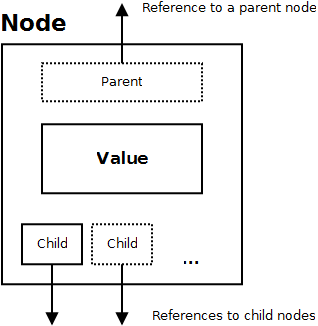
\includegraphics[width=0.4\columnwidth]{img/programming-fundamentals/node-general-model}
		\caption{A model for a node in a recursive data structure.}
		\label{fig:recursive-data-node}
	\end{center}
\end{figure}


Recursive data structures are usually dynamic, as adding, removing and inserting items can be done in constant time. The performance of finding elements in recursive data structures depends a lot on the type of query and the data structure itself, as we will see further.


\subsubsection{Linked lists}

A linked list is an ordered sequence of data elements contained in nodes. Nodes have a one-to-one parent-child relationship among them. The root node has no parent and the end node has no child. Traversing all the elements of a linked list occurs by starting at the root and each time going to the next element via the child reference of each node.

In general finding an item at a specific index requires linear time in worst case. However, by retaining certain meta-data, it is possible to add some speed-ups, of course at cost of memory usage and a performance cost to keep these additional fields up-to-date.

\begin{lstlisting}[language=java, caption=Node implementation for a linked list., label=listing:node-linked-list]
public class Node<E> {
	public E value;
	public Node next;
}
\end{lstlisting}


\paragraph{Doubly-linked list}


\paragraph{Circular linked list}




\subsubsection{Trees}

Trees can be seen as an extension of a linked list that can have more than one child. The root of the tree is the only element in the tree that has no parent element; all other elements have exactly one parent. Note that for this reason, a tree can never be circular. A node that has no children is called a leaf. The length longest path starting from the root and ending in a leaf, passing through a node at most once, is the height of the tree.


\paragraph{Binary trees}

A binary tree is a tree in which each node has at most two children.


\paragraph{Balanced trees}

In a balanced tree, all paths starting from the root and ending in a leaf node have equal length


\paragraph{Tries}

A trie is a specialized data structure in which for example letters are laid out along the paths of the tree, forming words. It allows certain algorithms to quickly find substrings within long sequences.


\subsection{Tuples}

A tuple is an ordered set of data elements. The elements are not necessarily all of the same type.



\section{Collections}

In what follows we discuss different APIs for collections. Table \ref{tab:api:collections} gives an overview of the general inspection methods for collections.

\begin{table}[H]
	\caption{General inspection methods for collections.}
	\label{tab:api:collections}
	\begin{tabular}{p{150px} | p{250px}}
		\textbf{Operation} & \textbf{Description} \\
		\hline
		size() $\rightarrow$ Integer & Returns the number of items in the collection. \\
		isEmpty() $\rightarrow$ Boolean & Returns $True$ if the number of items in the collection is zero. \\
		& \\
		\hline
	\end{tabular}
\end{table}



\subsection{Lists}

A list is an ordered sequence of data elements in which elements are allowed to occur more than once. Lists are typically mutable or dynamic, in the sense that items can be added to, replaced, and removed from it. There exist two notable variations to lists that differ in the way data is represented internally, namely array-based lists and linked lists.

where each data element is associated with an index. Table \ref{tab:api:list} gives an overview of the methods can can be invoked on a list. Note that some of the specification may change depending on certain design choices. For example, if the index is equal or greater than the length of the list, an error message could be shown. In this case the operation would simply have no effect.

\begin{table}[H]
	\caption{List API.}
	\label{tab:api:list}
	\begin{tabular}{p{150px} | p{250px}}
		\textbf{Operation} & \textbf{Description} \\
		\hline
		add($Item$) & Adds an item to the back of the list. \\
		get($index$) $\rightarrow$ $Item$ & Returns the item at the given index. \\
		replace($Item$, $index$) & Replaces the item at the given index in the list with the given item.  \\
		remove($index$) & Removes the item at the given index. \\
		\hline
	\end{tabular}
\end{table}



\subsection{Bags}

A bag is a collection that does not support the removal of items [2]. Only the adding of items and some inspection methods are generally supported. \textbf{Table} shows the bag API.

\begin{table}[H]
	\caption{Bag API.}
	\label{tab:api:bag}
	\begin{tabular}{p{150px} | p{250px}}
		\textbf{Operation} & \textbf{Description} \\
		\hline
		add($Item$) & Adds a new item to the bag. \\
		\hline
	\end{tabular}
\end{table}



\subsection{Queues}

\subsubsection{FIFO queues}

In its most common form, a queue is a data structure interface where items are added to the back and removed from the front of the internal array representation. This kind of policy is also called first-in-first-out (FIFO).

\begin{table}[H]
	\caption{Queue API.}
	\label{tab:api:queue}
	\begin{tabular}{p{150px} | p{250px}}
		\textbf{Operation} & \textbf{Description} \\
		\hline
		enqueue($Item$) & Places a new item at the end of the queue. \\
		dequeue() $\rightarrow$ $Item$ & Removes the first item from the queue and returns it. \\
		\hline
	\end{tabular}
\end{table}



\subsubsection{Priority queues}

A priority queue differs somewhat from a FIFO queue as both enqueue and dequeue method will have different effects. Each element has a priority associated with it that implies an inherent order among the elements. This may be as simple as alphabetic or numerical order, but may also involve multiple, more complex priorities. Usually this relationship among the elements is hidden from the data structure itself, and a simple compare method allows the data structure's algorithm to determine which element has priority over another element.

The semantantics of the dequeue method remain largely the same, except that the consistency within the queue has the be preserved. The enqueue method will not necessarily add a new element to the front of the queue. Instead, the elements have a priority associated with them, and the new element will be placed into the queue according to its priority with regard to the other queued elements. When the first element in the queue is removed, an algorithm has to determine which element should be the new first element. Again, depending on whether or not arrays or recursive data structures are, the algorithm will be different.



\subsection{Stacks}

A \emph{pushdown stack} is a data structure interface where items are added to and removed from the front of the internal array. This kind of policy is called \emph{last-in-first-out} (LIFO).

\begin{table}[H]
	\caption{Stack API.}
	\label{tab:api:stack}
	\begin{tabular}{p{150px} | p{250px}}
		\textbf{Operation} & \textbf{Description} \\
		\hline
		push($Item$) & Places a new item at the top of the stack. \\
		pop() $\rightarrow$ $Item$ & Removes the top item from the stack and returns it. \\
		\hline
	\end{tabular}
\end{table}



\section{Graphs}

Finally we will discuss graphs as another way to structure data. Graphs could be regarded as another recursive data type that is an extension of a tree, but instead of only allowing one parent, nodes have a many-to-many relationship among them, where edges define which nodes are connected. However, because of this additional "connector" we will discuss it here as a separate way of structuring data.

A graph consists of a set of nodes that are interconnected through a set of edges. In \textbf{table} the API for a general graph is shown. Graphs are commonly used to find path along the edges between different nodes. A path between nodes $v$ and $w$ is a an ordered list of edges where the first edge starts in $v$ and the last ends in $w$. In a fully connected graph, there exists a path between any pair of vertices. However, it may be possible that there exist more than one path between two vertices. This introduces some interesting problems, for example efficient algorithms have been developed to find the shortest path between two nodes.

\begin{table}[H]
	\caption{General graph API.}
	\label{tab:api:graph}
	\begin{tabular}{p{150px} | p{250px}}
		\textbf{Operation} & \textbf{Description} \\
		\hline
		addEdge($v$, $w$) & Adds a new edge with end points in vertices $v$ and $w$ to the graph. \\
		removeEdge($v$, $w$) & Removes an edge with end points in vertices $v$ and $w$ from the graph. \\
		findPath($v$,$w$,$Algorithm$)  $\rightarrow$ List<$Edge$> & Returns all the edges in a path, i.e., an ordered list of edges, between vertex $v$ and vertex $w$ using a given algorithm or policy. The result will depend on the algorithm that implements this method (e.g. path flooding, shortest path, ...). If no such path exists, an empty list is returned. \\
		\hline
	\end{tabular}
\end{table}

Formally a graph $G$ is defined as a tuple ($V$,$E$) where $V$ is the set of vertices or nodes and $E$ the set of edges. Every edge $e$ in $E$ is an pair ($v$,$w$) in $V x V$.


\subsection{Undirected graphs}

In an undirected graph the pair for edge $e$ = ($v$,$w$) is unordered, i.e., for every edge $e$ in $E$, the ordered pair ($v$,$w$) = ($w$,$v$). An important consequence of this is that when traversing the graph along a path from point A to B, you can always go in the opposite direction from B to A along the same path.

\begin{table}[H]
	\caption{Additional methods for undirected graphs.}
	\label{tab:api:graph-undirected}
	\begin{tabular}{p{150px} | p{250px}}
		\textbf{Operation} & \textbf{Description} \\
		\hline
		getEdges(v) $\rightarrow$ Bag<Edge> & Returns all the edges directly connected to a given vertex $v$. \\
		degree(v) $\rightarrow$ Bag<Edge> & Returns the number of edges directly connected to a given vertex $v$. \\
		\hline
	\end{tabular}
\end{table}



\subsection{Directed graphs}

In a directed graph $G$ = ($V$,$E$), an edge $e$ in $E$ is an ordered pair ($v$,$w$), denoting that a path exists from $v$ to $w$. However, the path in the opposite direction does not necessarily exist.







%\section{Tables}
% maps, key-value pairs, hash tables, tuples

